\documentclass[10pt,nofootinbib]{revtex4}
\usepackage{amsmath,amssymb,amsfonts,mathrsfs,bm,dsfont}
\usepackage[all]{xy}
\usepackage[normalem]{ulem}	% delete line
\usepackage{graphics,color}
\usepackage{tikz}
\usetikzlibrary{calc}
%\usepackage{hyperref}

\newcommand*\dd{\mathop{}\!\mathrm{d}}
\newcounter{Claim}[section]
\newenvironment{Claim}[1][]{{\par\normalfont\bfseries \underline{Claim~\stepcounter{Claim}\arabic{Claim}.}~#1~~}}{\par}
\newcounter{Proposition}[section]
\newenvironment{Proposition}[1][]{{\par\normalfont\bfseries \underline{Proposition~\stepcounter{Proposition}\arabic{Proposition}.}~#1~~}}{\par}
\newcounter{Note}[section]
\newenvironment{Note}[1][]{{\par\normalfont\bfseries \underline{Note~\stepcounter{Note}\arabic{Note}.}~#1~~}}{\par}
\newcounter{Lemma}[section]
\newenvironment{Lemma}[1][]{{\par\normalfont\bfseries \underline{Lemma~\stepcounter{Lemma}\arabic{Lemma}.}~#1~~}}{\par}
\newcounter{Corollary}[section]
\newenvironment{Corollary}[1][]{{\par\normalfont\bfseries \underline{Corollary~\stepcounter{Corollary}\arabic{Corollary}.}~#1~~}}{\par}
\newenvironment{Proof}{{\par~{\normalfont\bfseries $\vartriangleright$}~~}}{\hfill $\square$\par\hfill\par} %\par
\newcounter{Def}[section]
\newenvironment{Def}[1][]{{\par\normalfont\bfseries \underline{Definition~\stepcounter{Def}\arabic{Def}.}~#1~~}}{\par}

\allowdisplaybreaks[4] %允许 align 跨页编排

\def\Re{\mathop{\mathcal{R}e}}
\def\Im{\mathop{\mathcal{I}m}}

\newcommand\hexagon{\mathop{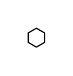
\begin{tikzpicture}[scale=0.06,baseline]
		\draw (0,-1) -- (1.732,0) -- (1.732,2) -- (0,3) -- (-1.732,2) -- (-1.732,0) -- (0,-1);
	\end{tikzpicture}}}



\begin{document}
\title{The Art of Guessing Hamiltonian in Honeycomb Lattice and Beyond}% Force line breaks with \\
%\thanks{This is a reminiscent note for Hubbard-Stratonovich Transformation.}%

\author{Xiaodong Hu}
%\altaffiliation[Also at ]{Boson College}
\email{xiaodong.hu@bc.edu}
\affiliation{Department of Physics, Boston College}

\date{\today}


\begin{abstract}
	This short practice is a reflection of the power of symmetry in contemporary condensed matter physics. We will try to find out all possible forms of allowed Hamiltonian of nearest neighbor level or even next nearest neighbot level with spin orbit coupling (SOC) in the honeycomb lattice (for instance, $\alpha$-$\mathrm{RuCl}_3$), and classify them with the help of representation theory of \emph{little group}. After that we will impose $t/U$ expansion to verify our results and try to express the electric polarization operator for nearest neightbor or even next nearest neighbot sites with spin degrees of freedom.
\end{abstract}
\maketitle
\tableofcontents
\section{Introduction}
	\subsection{Pure Hubbar Model}
		For \emph{pure} Hubbard model without spin-orbit coupling (SOC), Hamiltonian
		\begin{equation}\label{1.1.1}
			H=-t\sum_{\langle ij \rangle,\alpha}c_{i \alpha}^\dagger c_{j \alpha}+U\sum_i n_{i\uparrow}n_{i\downarrow}
		\end{equation}
		is invariant under \emph{global} $SU(2)$ spin-rotation symmetry $c_{i \alpha}\mapsto U_{\alpha \beta}c_{i \beta}$ as well as \emph{time-reversal symmetry}, \emph{parity symmetry}, and some specific \emph{cystalline symmetry}, depending on what kind of lattice we are working with.\par
		Throughout this paper, we only focus on honeycomb lattice, or more specifically, iridates family $A_2\mathrm{IrO_4}$ with $A=\mathrm{Na^{2+},Li^{2+}}$, which is believed to be the candidate realizing Kitaev spin chain \cite{kitaev2006anyons}. In this case the symmetry group is generated by two \emph{oblique-corssing} translation $T_1, T_2$, \emph{three-fold} rotation $C_3$, horizontal mirror symmetry $P$ and time-reversal symmtry $T$
		\begin{equation*}
			SG=\{T_1,T_2,C_3,P,T\}
		\end{equation*}
		with the confinement \cite{lu2010spin} on group elements
		\begin{align*}
			T^2=P^2=C_6^6&=1,\\
			TUT^{-1}U^{-1}&=1,\quad U=T_1,T_2,C_6,P,\\
			T_1T_2T_1^{-1}T_2^{-1}&=1,\\
			T_1^{-1}PT_1P&=1,\\
			T_2^{-1}PT_1T_2^{-1}P&=1,\\
			PC_6PC_6&=1,\\
			T_2^{-1}C_6T_1C_6&=1,\\
			T_1^{-1}C_6T_1T_2^{-1}C_6&=1.
		\end{align*}
		But how to use these spacial group? In fact, \textbf{given the coupling between arbitrary nearest neighbor links, one can immediately push it to all the other links of the lattice under the action of the spacial group we listed above. And because Hamiltonian is the summation of \emph{local} operators, we can fully recovered the Hamiltonian from such local details}. So the question of classifying \emph{pure} Hubbard Hamiltonian is narrowed to classifaction of the possible form of coupling on the link, say, the one between site $i$ and site $j$.

	\subsection{Spin Hamiltonian}
		Physical interesting things occur at \emph{half-filling} under \emph{strong-coupling limit}. But the first thing is to write down the low-energy effective Hamiltonian from \eqref{1.1.1}. Standard $t/U$ expansion will be discussed in the third section. In the first two sections, we try to guess the allowed form purely based on symmetric analysis.\par
		Under strong-coupling limit, each site is occupied by one electron \cite{Fradkin2013Field}. So by identifying $|n_{i\uparrow}=1\rangle\equiv|\uparrow\rangle$ and $|n_{i\downarrow}=1\rangle\equiv|\downarrow\rangle$ (this is certainly a one-to-one mapping), \textbf{one can always express the fermionic form of Hamiltonian with spin degree of freedom on each site} \cite{macdonald1988t}.\par
		Focusing on the nearest-neighbor $i$ and $j$, we have spin operator $\bm{S}_i$ and $\bm{S}_j$ in hand. The question is how to assembly them? One may naively say that there is no constaint so arbitrary form of coupling is OK. However, \textbf{no matter which order of perturbation we are working with, after decomposition and projection of many-body Hilbert space \cite{macdonald1988t,chernyshev2004higher}, we must end up with the combinations of terms holding the same symmetry as original Hamiltonian}. And because original Hubbard Hamiltonian is invariant under $SU(2)$ spin-rotation, so should our low-energy effective Hamiltonian be under the strong-coupling limit. All the other forms of assembly are forbidden by symmetry, except for 
		\begin{equation*}
			H_{ij}\propto\bm{S}_i\cdot\bm{S}_j
		\end{equation*}
		because of the strong dependence of the identity $\bm{\sigma}_{\alpha \beta}\cdot\bm{\sigma}_{\mu\nu}=2\delta_{\alpha\nu}\delta_{\beta\mu}-\delta_{\alpha \beta}\delta_{\mu\nu}$, ensuring
		\begin{equation*}
			\bm{S}_i\cdot\bm{S}_j=\sum_{\alpha \beta \mu \nu}c_{i \alpha}^\dagger\dfrac{\bm{\sigma}_{\alpha \beta}}{2}c_{i \beta}\cdot c_{j \mu}^\dagger\dfrac{\bm{\sigma}_{\mu\nu}}{2}c_{j \mu}=\text{simple combinations of four fermionic operators},
		\end{equation*}
		which is explicitly invariant under spin rotations.
	
	\subsection{Spin-orbit Coupling}
		It is the \emph{independence} of spin-rotational symmetry and crystalline symmetry for the original Hamiltonian \eqref{1.1.1} that extremely simplify our work of classification (as is shown above, there is merely one kind allowed).\par
		But when SOC starts to play the role in Hamiltonian, say
		\begin{equation}\label{1.2.1}
			H_{\text{SOC}}=\lambda\bm{L}\cdot\bm{S},
		\end{equation}
		all the discussion break down because now spin-rotational symmetry \emph{couple with} crystalline symmetry in the sense that, if we have known the local Hamiltonian $H_{ij}$ on one link $i,j$ and want to push it by rotation, inversion, and translation as we have done before, then unfortunately the spin form of $H_{ij}$ will also be altered. For example, in Kitaev spin chain \cite{kitaev2006anyons}, if the local Hamiltonian for one link is given, say, $S_i^xS_j^x$, then after $\pi/3$ and $2\pi/3$ rotations, we end up with $S_i^yS_k^y$ and $S_i^zS_\ell^z$ respectively. They are no longer the same.


\section{Classification of Hamiltonian}
	At the nearest-neighbor level, Hamiltonian can be generally expressed as
	\begin{equation}\label{2.0.1}
		H=\sum_{\hexagon}\sum_{\langle ij \rangle\in\hexagon}\gamma_{\mu\nu}^{\langle ij \rangle }S_i^\mu S_j^\nu.
	\end{equation}
	where $\gamma_{\mu\nu}$ are complex coefficient waiting to be determined by symmetry. We will start with classifying Hamiltonian on one link
	\begin{equation}\label{2.0.2}
		H_{ij}=\gamma_{\mu\nu}^{\langle ij \rangle }S_i^\mu S_{j}^\nu.
	\end{equation}
	\subsection{Hamiltonian on a Link}
		Although SOC term leads orbital rotation coupling with spin rotation, time-reversal symmetry as well as parity inversion symmetry still survive for $H_{ij}$. In terms of group action on group representation, we have
		\begin{equation}\label{2.1.1}
			\rho(g) H_{ij}\rho^\dagger(g)=H
		\end{equation}
		for $g=T$ or $P$, giving
		\begin{align}
			\rho(T) H_{ij}\rho^\dagger(T)&={\gamma_{\mu\nu}^{\langle ij \rangle }}^*(-S_i^\mu)(-S_j^\nu)\equiv H_{ij}\implies{\gamma^{\langle ij \rangle}_{\mu\nu}}^*\equiv\gamma_{\mu\nu}^{\langle ij \rangle },\label{2.1.2}\\
			\rho(P) H_{ij}\rho^\dagger(P)&=\gamma_{\mu\nu}^{\langle ij \rangle }S_j^\mu S_i^\nu\equiv H_{ij}\implies\gamma_{\mu\nu}^{\langle ij \rangle }\equiv\gamma_{\nu\mu}^{\langle ij \rangle },\label{2.1.3}
		\end{align}
		respectively. Therefore, coefficient matrix $\gamma$ is \emph{real} and \emph{symmetric}.\par
		But this is far less the end of the story. In fact, when we include the entire space group of our $\mathrm{A_2IrO_3}$ lattice, there is one more group action keeping the link $ij$ unchanged --- the (spin) rotation along local $\hat{Y}$ direction, or global $\dfrac{1}{\sqrt{2}}(-\hat{x}+\hat{y})$ direction. This is clear from the two octahedral structures in FIG \ref{fig:Link}.\par
		\begin{figure}[!htp]
			\centering
			\includegraphics[scale=0.1]{Link.pdf}
			\caption{{\bf Ir-Ir Link}: For each link we assign a local (purple) frame with $\hat{Y}$ in Ir-Ir direction and global spin (yellow) frame pointing three orthogonal Ir-O directions of an octahedra.}
			\label{fig:Link}
		\end{figure}
		Therefore, if we express $\gamma$ matrix in local spin frame (and denote it as $\widetilde{\gamma}_{\mu\nu}$), then because
		\begin{equation*}
			\left(\begin{array}{ccc}
				-1 & 0 & 0 \\ 0 & 1 & 0 \\ 0 & 0 & -1
			\end{array}\right)\widetilde{\gamma}_{\mu\nu}^{\langle ij \rangle }
			\left(\begin{array}{ccc}
				-1 & 0 & 0 \\ 0 & 1 & 0 \\ 0 & 0 & -1
			\end{array}\right)\equiv\widetilde{\gamma}_{\mu\nu}^{\langle ij \rangle }
		\end{equation*}

		\noindent we can only write
		\begin{equation}\label{2.1.4}
			\widetilde{\gamma}_{\mu\nu}^{\langle ij \rangle }=\left(\begin{array}{ccc}
				A & 0 & D \\ 0 & B & 0 \\ D & 0 & C
			\end{array}\right).
		\end{equation}
		\indent For further discussion of orbital rotation, it's helpful to go back to global spin frame (so that the coupling of spin rotation with orbital rotation is definitely decided)
		\begin{equation*}
			\widetilde{\bm{S}}=P\bm{S},\text{ or }\left(\begin{array}{c}
				\widetilde{S}^X \\ \widetilde{S}^Y \\ \widetilde{S}^Z
			\end{array}\right)=\left(\begin{array}{ccc}
				1/\sqrt{2} & 1/\sqrt{2} & 0\\-1/\sqrt{2} & 1/\sqrt{2} & 0\\ 0 & 0 & 1
			\end{array}\right) \left(\begin{array}{c}
				S^x \\ S^y \\ S^z
			\end{array}\right).
		\end{equation*}
		So
		\begin{equation}\label{2.1.5}
			\gamma_{\mu\nu}^{\langle ij \rangle }=\left(\begin{array}{ccc}
				\frac{a}{2}+\frac{b}{2} & \frac{b}{2}-\frac{a}{2} & \frac{d}{\sqrt{2}} \\
				\frac{b}{2}-\frac{a}{2} & \frac{a}{2}+\frac{b}{2} & \frac{d}{\sqrt{2}} \\
				\frac{d}{\sqrt{2}} & \frac{d}{\sqrt{2}} & c
			\end{array}\right)
		\end{equation}
		and
		\begin{equation}\label{2.1.6}
			H_{ij}=J_{ij}\bm{S}_i\cdot\bm{S}_j+K_{ij}S_i^zS_j^z+\Gamma_{ij}(S_i^xS_j^y+S_i^yS_j^x)+\Gamma'_{ij}(S_i^xS_j^z+S_i^zS_j^x+S_i^yS_j^z+S_i^zS_j^y),
		\end{equation}
		where for physical reason Heisenberg-like term is splitted out and
		\begin{equation*}
			J_{ij}\equiv\dfrac{a+b}{2},\quad K_{ij}\equiv c-\dfrac{a+b}{2},\quad \gamma_{ij}\equiv\dfrac{b-a}{2},\quad \Gamma'_{ij}\equiv\dfrac{d}{\sqrt{2}}.
		\end{equation*}
		This result is in consistent with $t/U$ expansion study of \cite{rau2014generic}, chemical calculation of \cite{katukuri2014kitaev}, and first-principle study of \cite{hu2015first}. 
	\subsection{Hamiltonian on the Entire Lattice}
		We are interested in the trivial representation of translation transformation, i.e.,
		\begin{equation*}
			\rho(T_1)S_i^\mu\rho^\dagger(T_1)\equiv S_{T_1^{-1}(i)}^\mu,\quad \rho(T_2)S_i^\mu\rho^\dagger(T_2)\equiv S_{T_2^{-1}(i)}^\mu,
		\end{equation*}
		So the left work of classification of Hamiltonian can be concentrated to the discussion of the honeycomb
		\begin{equation}\label{2.2.1}
			H_{\hexagon}\equiv\sum_{\langle ij \rangle \in\hexagon}\gamma_{\mu\nu}^{\langle ij \rangle }S_i^\mu S_j^\nu.
		\end{equation}
		Fortunately, once global spin orientation is chosen, the coupling of orbital rotation with spin rotation is no longer ambiguous and can be read directly from FIG. \ref{fig:hexagon}.
		\begin{figure}[!htp]
			\centering
			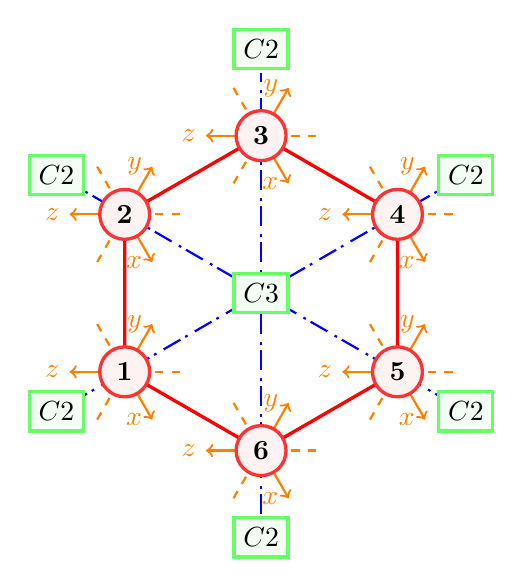
\begin{tikzpicture}[scale=1,baseline]
				\coordinate (a) at (0,0);
				\coordinate (b) at (1.732,1);
				\coordinate (c) at (1.732,3);
				\coordinate (d) at (0,4);
				\coordinate (e) at (-1.732,3);
				\coordinate (f) at (-1.732,1);

				\draw[red,very thick] (a) -- (b) -- (c) -- (d) -- (e) -- (f) -- cycle;
				
				\draw[thick,orange,rotate around={180:(a)},dashed] ($(-0.7,0)+(a)$)--($(0,0)+(a)$);
				\draw[->,thick,orange,rotate around={180:(a)}] ($(0,0)+(a)$)--($(0.7,0)+(a)$) node[left]{$z$};
				\draw[thick,orange,rotate around={60:(a)},dashed] ($(-0.7,0)+(a)$)--($(0,0)+(a)$);
				\draw[->,thick,orange,rotate around={60:(a)}] ($(0,0)+(a)$)--($(0.7,0)+(a)$) node[left]{$y$};
				\draw[thick,orange,rotate around={-60:(a)},dashed] ($(-0.7,0)+(a)$)--($(0,0)+(a)$);
				\draw[->,thick,orange,rotate around={-60:(a)}] ($(0,0)+(a)$)--($(0.7,0)+(a)$) node[left]{$x$};

				\draw[thick,orange,rotate around={180:(b)},dashed] ($(-0.7,0)+(b)$)--($(0,0)+(b)$);
				\draw[->,thick,orange,rotate around={180:(b)}] ($(0,0)+(b)$)--($(0.7,0)+(b)$) node[left]{$z$};
				\draw[thick,orange,rotate around={60:(b)},dashed] ($(-0.7,0)+(b)$)--($(0,0)+(b)$);
				\draw[->,thick,orange,rotate around={60:(b)}] ($(0,0)+(b)$)--($(0.7,0)+(b)$) node[left]{$y$};
				\draw[thick,orange,rotate around={-60:(b)},dashed] ($(-0.7,0)+(b)$)--($(0,0)+(b)$);
				\draw[->,thick,orange,rotate around={-60:(b)}] ($(0,0)+(b)$)--($(0.7,0)+(b)$) node[left]{$x$};

				\draw[thick,orange,rotate around={180:(c)},dashed] ($(-0.7,0)+(c)$)--($(0,0)+(c)$);
				\draw[->,thick,orange,rotate around={180:(c)}] ($(0,0)+(c)$)--($(0.7,0)+(c)$) node[left]{$z$};
				\draw[thick,orange,rotate around={60:(c)},dashed] ($(-0.7,0)+(c)$)--($(0,0)+(c)$);
				\draw[->,thick,orange,rotate around={60:(c)}] ($(0,0)+(c)$)--($(0.7,0)+(c)$) node[left]{$y$};
				\draw[thick,orange,rotate around={-60:(c)},dashed] ($(-0.7,0)+(c)$)--($(0,0)+(c)$);
				\draw[->,thick,orange,rotate around={-60:(c)}] ($(0,0)+(c)$)--($(0.7,0)+(c)$) node[left]{$x$};

				\draw[thick,orange,rotate around={180:(d)},dashed] ($(-0.7,0)+(d)$)--($(0,0)+(d)$);
				\draw[->,thick,orange,rotate around={180:(d)}] ($(0,0)+(d)$)--($(0.7,0)+(d)$) node[left]{$z$};
				\draw[thick,orange,rotate around={60:(d)},dashed] ($(-0.7,0)+(d)$)--($(0,0)+(d)$);
				\draw[->,thick,orange,rotate around={60:(d)}] ($(0,0)+(d)$)--($(0.7,0)+(d)$) node[left]{$y$};
				\draw[thick,orange,rotate around={-60:(d)},dashed] ($(-0.7,0)+(d)$)--($(0,0)+(d)$);
				\draw[->,thick,orange,rotate around={-60:(d)}] ($(0,0)+(d)$)--($(0.7,0)+(d)$) node[left]{$x$};

				\draw[thick,orange,rotate around={180:(e)},dashed] ($(-0.7,0)+(e)$)--($(0,0)+(e)$);
				\draw[->,thick,orange,rotate around={180:(e)}] ($(0,0)+(e)$)--($(0.7,0)+(e)$) node[left]{$z$};
				\draw[thick,orange,rotate around={60:(e)},dashed] ($(-0.7,0)+(e)$)--($(0,0)+(e)$);
				\draw[->,thick,orange,rotate around={60:(e)}] ($(0,0)+(e)$)--($(0.7,0)+(e)$) node[left]{$y$};
				\draw[thick,orange,rotate around={-60:(e)},dashed] ($(-0.7,0)+(e)$)--($(0,0)+(e)$);
				\draw[->,thick,orange,rotate around={-60:(e)}] ($(0,0)+(e)$)--($(0.7,0)+(e)$) node[left]{$x$};

				\draw[thick,orange,rotate around={180:(f)},dashed] ($(-0.7,0)+(f)$)--($(0,0)+(f)$);
				\draw[->,thick,orange,rotate around={180:(f)}] ($(0,0)+(f)$)--($(0.7,0)+(f)$) node[left]{$z$};
				\draw[thick,orange,rotate around={60:(f)},dashed] ($(-0.7,0)+(f)$)--($(0,0)+(f)$);
				\draw[->,thick,orange,rotate around={60:(f)}] ($(0,0)+(f)$)--($(0.7,0)+(f)$) node[left]{$y$};
				\draw[thick,orange,rotate around={-60:(f)},dashed] ($(-0.7,0)+(f)$)--($(0,0)+(f)$);
				\draw[->,thick,orange,rotate around={-60:(f)}] ($(0,0)+(f)$)--($(0.7,0)+(f)$) node[left]{$x$};


				\draw[dash pattern={on 7pt off 2pt on 1pt off 3pt},thick,blue,rotate around={0:(0,2)}] (0,-0.8)--(0,4.8);
				\draw[dash pattern={on 7pt off 2pt on 1pt off 3pt},thick,blue,rotate around={60:(0,2)}] (0,-0.8)--(0,4.8);
				\draw[dash pattern={on 7pt off 2pt on 1pt off 3pt},thick,blue,rotate around={-60:(0,2)}] (0,-0.8)--(0,4.8);
				\node[draw=green!60,fill=green!5,very thick,minimum size=5mm] at (2.6,3.5) {$C2$};
				\node[draw=green!60,fill=green!5,very thick,minimum size=5mm] at (2.6,0.5) {$C2$};
				\node[draw=green!60,fill=green!5,very thick,minimum size=5mm] at (0,-1.1) {$C2$};
				\node[draw=green!60,fill=green!5,very thick,minimum size=5mm] at (0,5.1) {$C2$};
				\node[draw=green!60,fill=green!5,very thick,minimum size=5mm] at (-2.6,3.5) {$C2$};
				\node[draw=green!60,fill=green!5,very thick,minimum size=5mm] at (-2.6,0.5) {$C2$};

				%\draw[->,dashed,very thick,green] (-0.4,1.8) .. controls (-0.6,2.6) and (0.6,2.6).. (0.4,1.8);
				\node[rectangle,draw=green!60,fill=green!5,very thick,minimum size=5mm] at (0,2) {$C3$};

				\node[circle,draw=red!80,fill=red!5,very thick,minimum size=5mm] at (a) {$\mathbf{6}$};
				\node[circle,draw=red!80,fill=red!5,very thick,minimum size=5mm] at (f) {$\mathbf{1}$};
				\node[circle,draw=red!80,fill=red!5,very thick,minimum size=5mm] at (e) {$\mathbf{2}$};
				\node[circle,draw=red!80,fill=red!5,very thick,minimum size=5mm] at (d) {$\mathbf{3}$};
				\node[circle,draw=red!80,fill=red!5,very thick,minimum size=5mm] at (c) {$\mathbf{4}$};
				\node[circle,draw=red!80,fill=red!5,very thick,minimum size=5mm] at (b) {$\mathbf{5}$};
			\end{tikzpicture}
			\caption{{\bf Global Spin Orientation on a Hexagon}: SOC term makes C2 rotation and C3 rotation along each Ir }
			\label{fig:hexagon}
		\end{figure}

		For instance, if we focus on link $\mathrm{Ir}_1\text{-}\mathrm{Ir}_2$ in FIG. \ref{fig:hexagon}, then $C_3$ rotation will transform it to link $\mathrm{Ir}_3\text{-}\mathrm{Ir}_4$, in which
		\begin{equation}\label{2.2.2}
			\rho(C_3)S_i^x\rho^\dagger(C_3)=S_{C_3(i)}^z,\quad \rho(C_3)S_i^y\rho^\dagger(C_3)=S_{C_3(i)}^x,\quad \rho(C_3)S_i^z\rho^\dagger(C_3)=S_{C_3(i)}^y.
		\end{equation}
		Unlike above $C_3$ rotation just connecting two links, $C_2$ rotation along $\mathrm{Ir}_2\text{-}\mathrm{Ir}_5$ axis will connect $\mathrm{Ir}_1\text{-}\mathrm{Ir}_2$ with $\mathrm{Ir}_3\text{-}\mathrm{Ir}_2$, $\mathrm{Ir}_6\text{-}\mathrm{Ir}_1$ with $\mathrm{Ir}_4\text{-}\mathrm{Ir}_3$, and $\mathrm{Ir}_5\text{-}\mathrm{Ir}_6$ with $\mathrm{Ir}_5\text{-}\mathrm{Ir}_4$. Still taking Link $\mathrm{Ir}_1\text{-}\mathrm{Ir}_2$ as example, we have
		\begin{subequations}
			\begin{align}
				\rho(C_2)S_2^x\rho^\dagger(C_2)&=-S_2^x,&\rho(C_2)S_1^x\rho^\dagger(C_2)&=-S_3^z,\label{2.2.3(a)}\\
				\rho(C_2)S_2^y\rho^\dagger(C_2)&=-S_2^y,&\rho(C_2)S_1^y\rho^\dagger(C_2)&=-S_3^y,\label{2.2.3(b)}\\
				\rho(C_2)S_2^z\rho^\dagger(C_2)&=-S_2^z,&\rho(C_2)S_1^z\rho^\dagger(C_2)&=-S_3^x.\label{2.2.3(c)}
			\end{align}
		\end{subequations}
		Therefore, we conclude that coefficients in \eqref{2.1.6} are the same for all the links. Namely,
		\begin{equation}\label{2.2.4}
			H_{\hexagon}=\sum_{\langle ij \rangle\in\hexagon}J\bm{S}_i\cdot\bm{S}_j+KS_i^zS_j^z+\Gamma(S_i^xS_j^y+S_i^yS_j^x)+\Gamma'(S_i^xS_j^z+S_i^zS_j^x+S_i^yS_j^z+S_i^zS_j^y).
		\end{equation}

\iffalse
		\subsection{Independent Time Time-reversal, Translation Symmetry, and $D_2$ Point Group}
			Although SOC term leads lattice rotation ($C_3$ for $\mathrm{A_2Ir_2O_4}$) coupling with spin rotation, time-reversal symmetry, lattice translation symmetry, as well as $D_{2h}$ point group symmetry on each link $i,j$ are still \emph{independent}. That is,
			\begin{equation}\label{2.1.1}
				TH_{ij}T^{-1}=H_{ij},\quad T_{1}H_{ij}T_{1}^{-1}=H_{ij},\quad T_{2}H_{ij}T_{2}^{-1}=H_{ij},
			\end{equation}
			and
			\begin{equation}\label{2.1.2}
				U(g) H_{ij}U^\dagger(g)=H,\quad g\in D_{2h}.
			\end{equation}
			Point group $D_{2h}$ is easy to see from {\color{red}FIG ???}, the two-octahedra cluster encompassing link $i,j$ of Ir atoms taken from the ideal cystal (without any distortion).\par
			Time-reversal symmetry gurantees $\gamma_{\mu\nu}$ is \emph{real}, parity inversion (in $D_{2h}$) through the link center $i,j$ tells us $\gamma_{\mu\nu}$ is \emph{symmetric}, plus the three two-fold rotation symmetry in $[110],[\bar{1}10]$, and $[001]$ direction in local spin frame, we can drastically simplify the coefficient, re-writting \eqref{2.0.1} as
			\begin{equation}\label{2.1.3}
				H_{ij}=J\bm{S}_i\cdot\bm{S}_j+\gamma_{\mu\nu} \widetilde{S_i^\mu}\widetilde{S_j^\mu},
			\end{equation}
			where $\widetilde{S_i^\mu}$ are spin operators defined on \emph{\color{red}local spin frames} (so just like the case in differential manifolds,\textbf{even if all corresponding components of two spin vectors in the spin space on \emph{distinct} sites coincides, we cannot say that they points at the same direction}, although all of them are isomorphic to $\mathbb{R}^3$) and $\gamma_{\mu\nu}$ has the form of
			\begin{equation}\label{2.1.3}
				\gamma_{\mu\nu}=\left(\begin{array}{ccc}
					A & 0 & 0 \\ 0 & B & C \\ 0 & C & -A-B
				\end{array}\right).
			\end{equation}
			$\gamma_{\mu\nu}$ is \emph{traceless} since we have explicitly splitted out the Heisenberg term at first for physical reasons.

		\subsection{Coupled Spin and Lattice Rotational Symmetry}
			Equation \eqref{2.1.2}, on the other hand, tells us that if we have known \emph{all six links} of Hamiltonian $H_{\hexagon}$ on each honeycomb, then by translation transformation we can generate the entire Hamiltonian on the lattice.
			Lattice structure of $A_2\mathrm{Sr_2O_3}$ is shown in FIG. \ref{fig:A2SrO3}. Because of SOC term in Hamiltonian, physical allowed $C_3$ rotation of each $\mathrm{Sr}$ atom demands a local rotation of spin frame at first to ensure one spin axis of each tetrahedra parallelling with the orbital rotation axis (and then recover with the proper orientation on new sites), which is represented by modification of the orientation of each tetrahedra.\par
			More specifihcally, 
			\begin{figure}[!htp]
				\centering
				\includegraphics[scale=0.7]{A2SrO3.pdf}
				\caption{{\bf Lattice Structure of $\mathbf{A_2SrO_3}$}: Clearly because of the staggered orientation of the oxygen tetrahedra, each $C_3$ rotation results in the switch of $S_i^x$ (or $S_i^y$) with $S_j^y$ (or $-S_j^x$).}
				\label{fig:A2SrO3}
			\end{figure}
\fi

\section{Electric Polarization Operator}
	%\subsection{Polarization on a Link}
		Unlike Hamiltonian, polarization operator is \emph{odd} under parity inversion of bond center. Therefore with the same time-reveral symmetry, we can write 
		\begin{equation}\label{3.1.1}
			P_{ij}=\lambda^{\langle ij \rangle }_{\mu\nu}S_i^\mu S_j^\nu
		\end{equation}
		with real but antisymmetric coefficient matrix
		\begin{equation*}
			\lambda_{\mu\nu}=\left(\begin{array}{ccc}
				0 & A & B \\ -A & 0 & C \\ -B & -C & 0
			\end{array}\right).
		\end{equation*}
		To analyze symmetry allowed form of polarization operator, we still start from a link and classify with little group action. For $C2$ rotation along $\hat{Z}$ direction,
		\begin{equation*}
			\left(\begin{array}{ccc}
				-1 & 0 & 0 \\ 0 & 1 & 0 \\ 0 & 0 & -1
			\end{array}\right)\widetilde{\lambda}_{\mu\nu}^{\langle ij \rangle }
			\left(\begin{array}{ccc}
				-1 & 0 & 0 \\ 0 & 1 & 0 \\ 0 & 0 & -1
			\end{array}\right)\equiv\widetilde{\lambda}_{\mu\nu}^{\langle ij \rangle }
		\end{equation*}
		gives
		\begin{equation}\label{3.1.2}
			\widetilde{\lambda}_{\mu\nu}^{\langle ij \rangle }=\left(\begin{array}{ccc}
				0&0&A\\0&0&0\\-A&0&0
			\end{array}\right).
		\end{equation}
		In global spin frame,
		\begin{equation}\label{3.1.3}
			\lambda_{\mu\nu}^{\langle ij \rangle }=\left(
			\begin{array}{ccc}
			 0 & 0 & \frac{A}{\sqrt{2}} \\
			 0 & 0 & \frac{A}{\sqrt{2}} \\
			 -\frac{A}{\sqrt{2}} & -\frac{A'}{\sqrt{2}} & 0 \\
			\end{array}
			\right)
		\end{equation}
		So
		\begin{equation*}
			P_{ij}=\dfrac{A}{\sqrt{2}}(S_i^xS_j^z-S_i^zS_j^x+S_i^yS_j^z-S_i^zS_j^y),
		\end{equation*}
		or in a more compact form
		\begin{equation}\label{3.1.4}
			P_{ij}=A(\bm{S}_i\times\bm{S}_j)\cdot\hat{\bm{e}}_{ij},
		\end{equation}
		where $\hat{\bm{e}_{ij}}$ is identified with $\hat{\bm{e}_{ij}}$ in FIG. \ref{fig:hexagon} so that $\hat{\bm{e}_{ij}}\equiv\dfrac{1}{\sqrt{2}}(-\hat{y}+\hat{z})$.\par
		With the same discussion on the remaining $C_3$ rotation and $C_2$ rotation (and trivial $T_1$ and $T_2$ translation) transformation, we can easily push $P_{12}$ to the entire lattice. Finally, we obtain
		\begin{equation}\label{3.1.5}
			P_{\hexagon}\equiv\sum_{\langle ij \rangle \in\hexagon}P_{ij}=A\sum_{\langle ij \rangle \in \hexagon}(\bm{S}_i\times\bm{S}_j)\cdot\hat{\bm{e}_{ij}}.
		\end{equation}
		This result is in consistent with that in \cite{bolens2018mechanism}.

\section{$t/U$ Expansion}
	But this is exactly true only if $t/U\rightarrow\infty$. In reality where $t$ is small but finite, chances are electrons hopping among sites and forming doubly occupied states.


\bibliography{hxd}
\bibliographystyle{apsrev} % apsrev is format for PRL of APS
\end{document}